\section{Scan Chain Architecture}
\label{sec:scanchain_arch}

Tiny Tapeout started as an experiment in fitting as many designs as possible into the \qty{10}{\milli\meter\squared} available on the Google lottery shuttles (Fig.~\ref{fig:500_designs_chain_TT01}).
As a fast proof of concept, a scan chain was chosen.
Each design had 8 inputs and 8 outputs.
Clock and reset were optional and not treated specially. The chain was formed of scan flops~\cite{skywaterpdk}, a type of flip flop with an integrated multiplexer at its input. An example showing a two-design scan chain is shown in Fig.~\ref{fig:simplified_view_2_designs}.

\begin{figure}[!t]
\centering
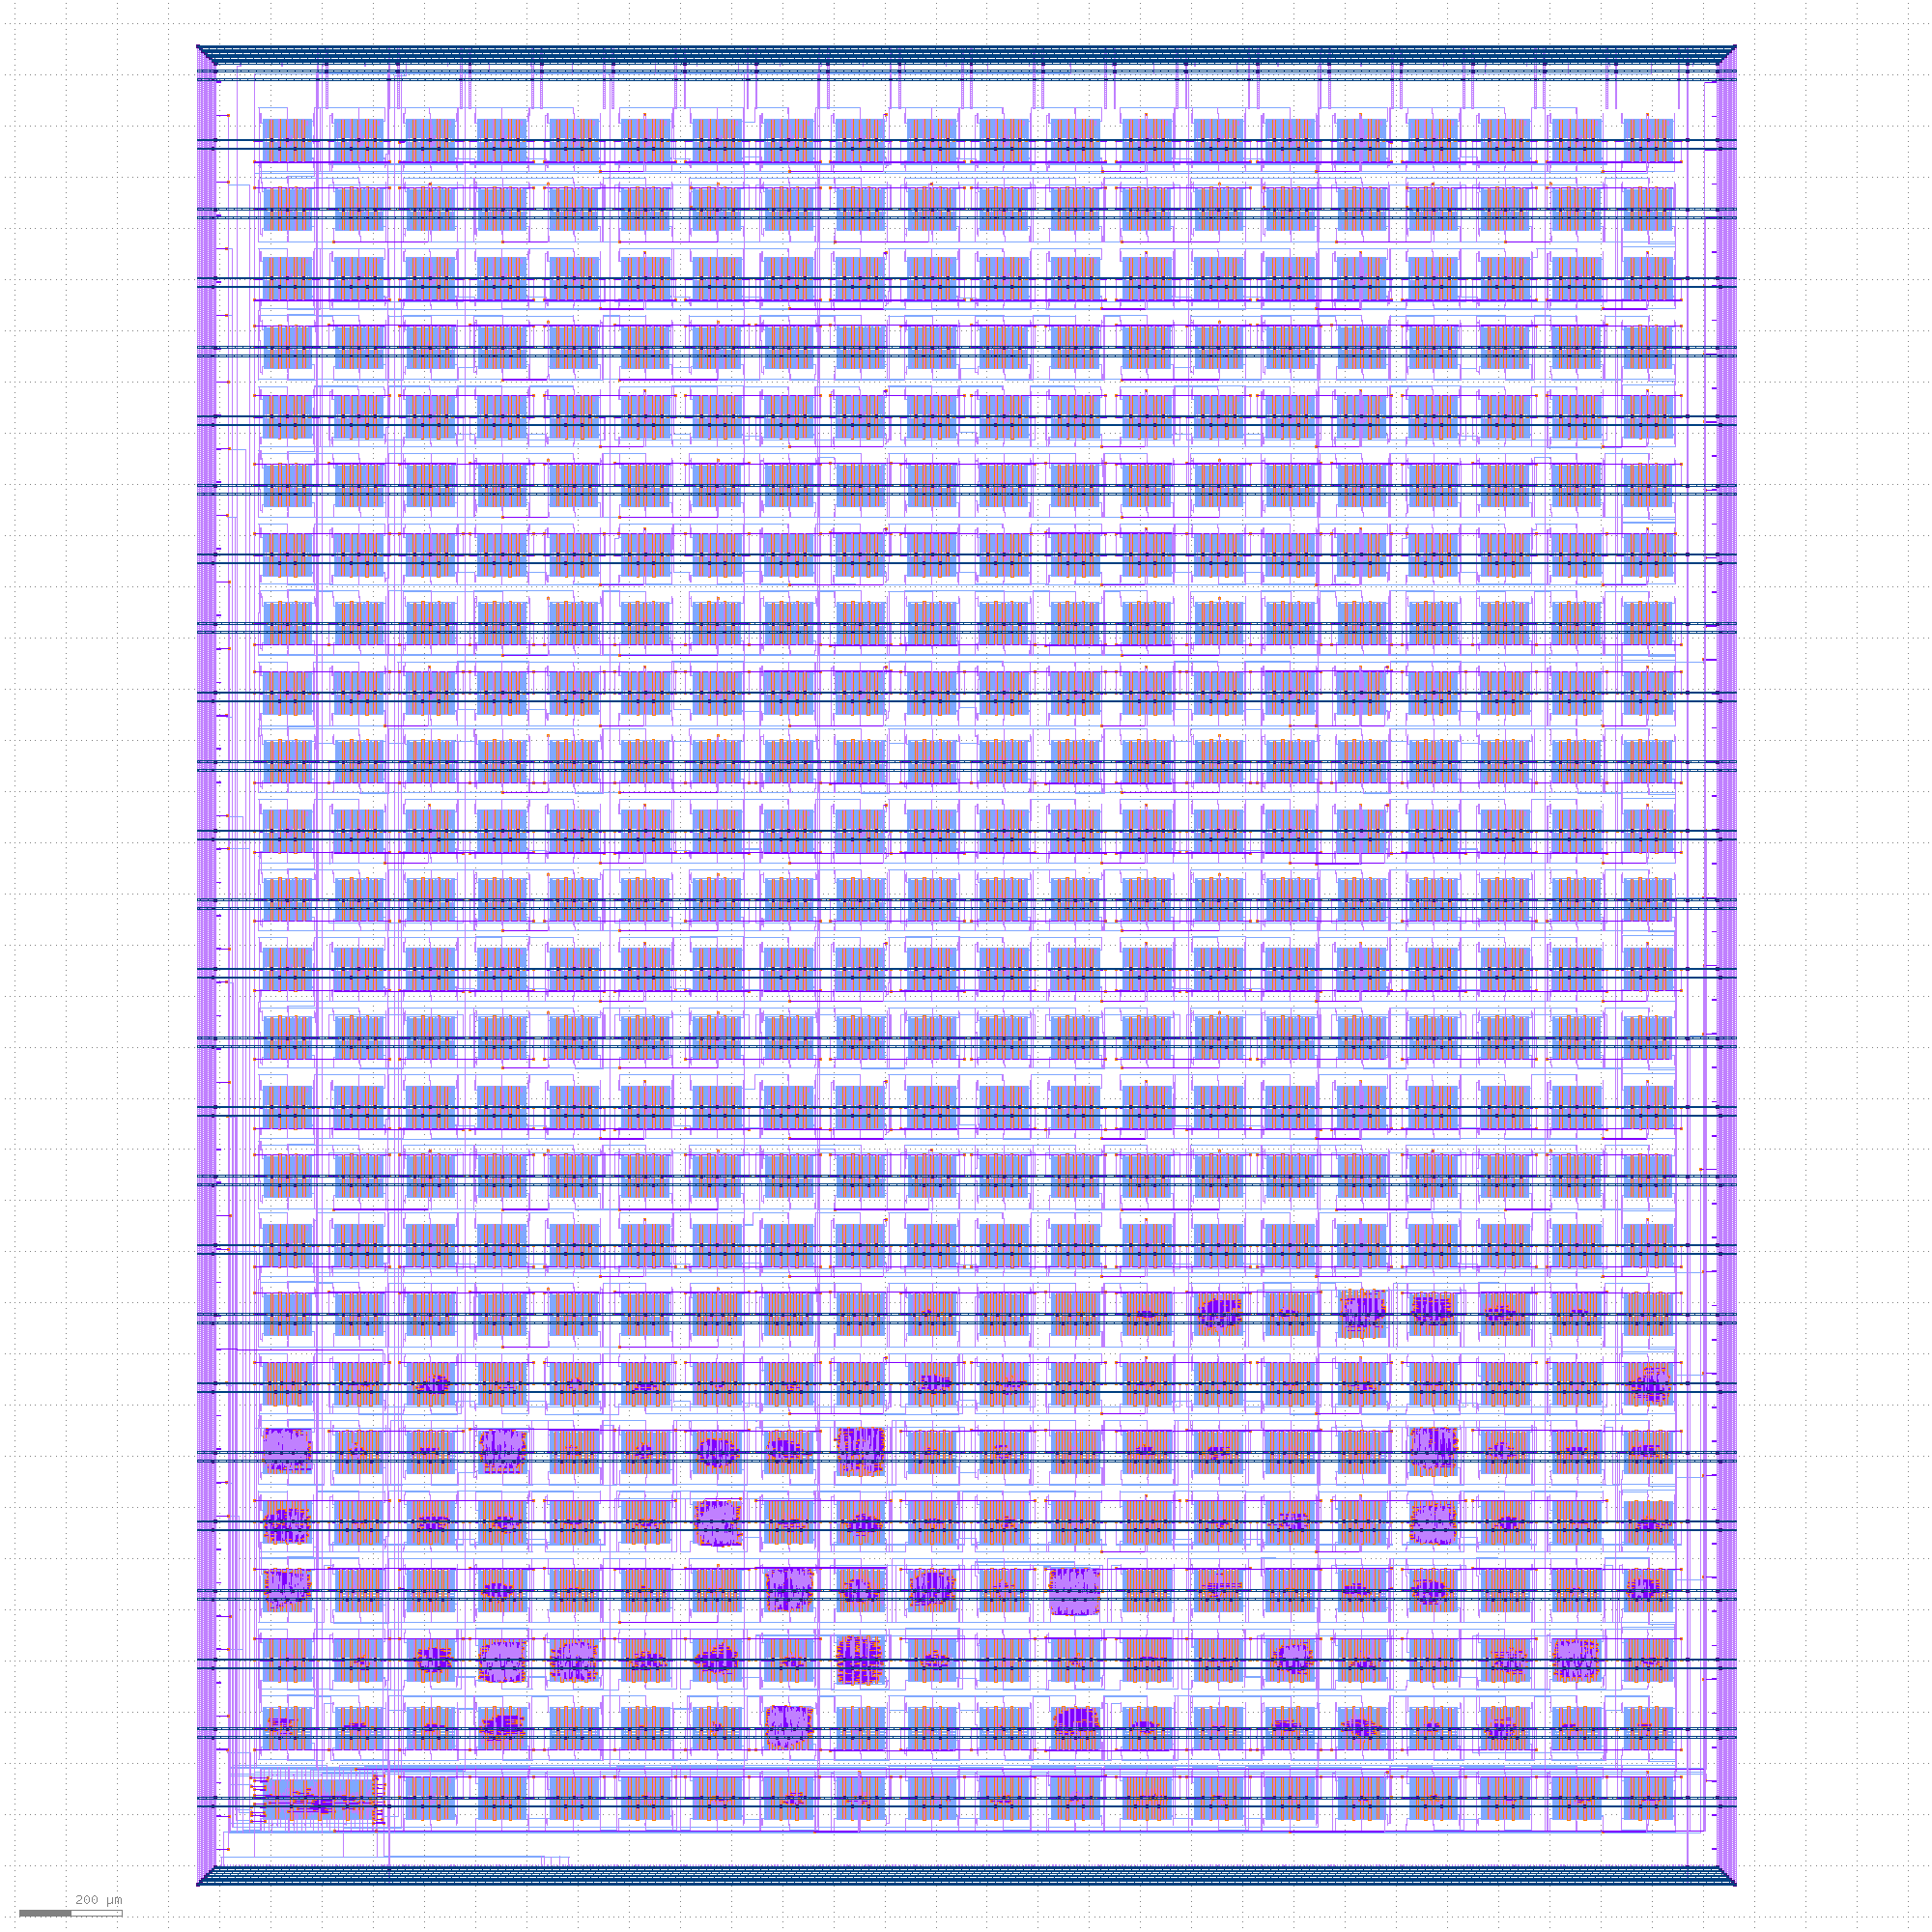
\includegraphics[width=1\columnwidth]{./Figs/tt01_whole_die.png}
\caption{500 designs connected in a chain for TT01, with the scan chain driver in the lower left corner.}
\label{fig:500_designs_chain_TT01}
\end{figure}

\begin{figure}[!t]
\centering
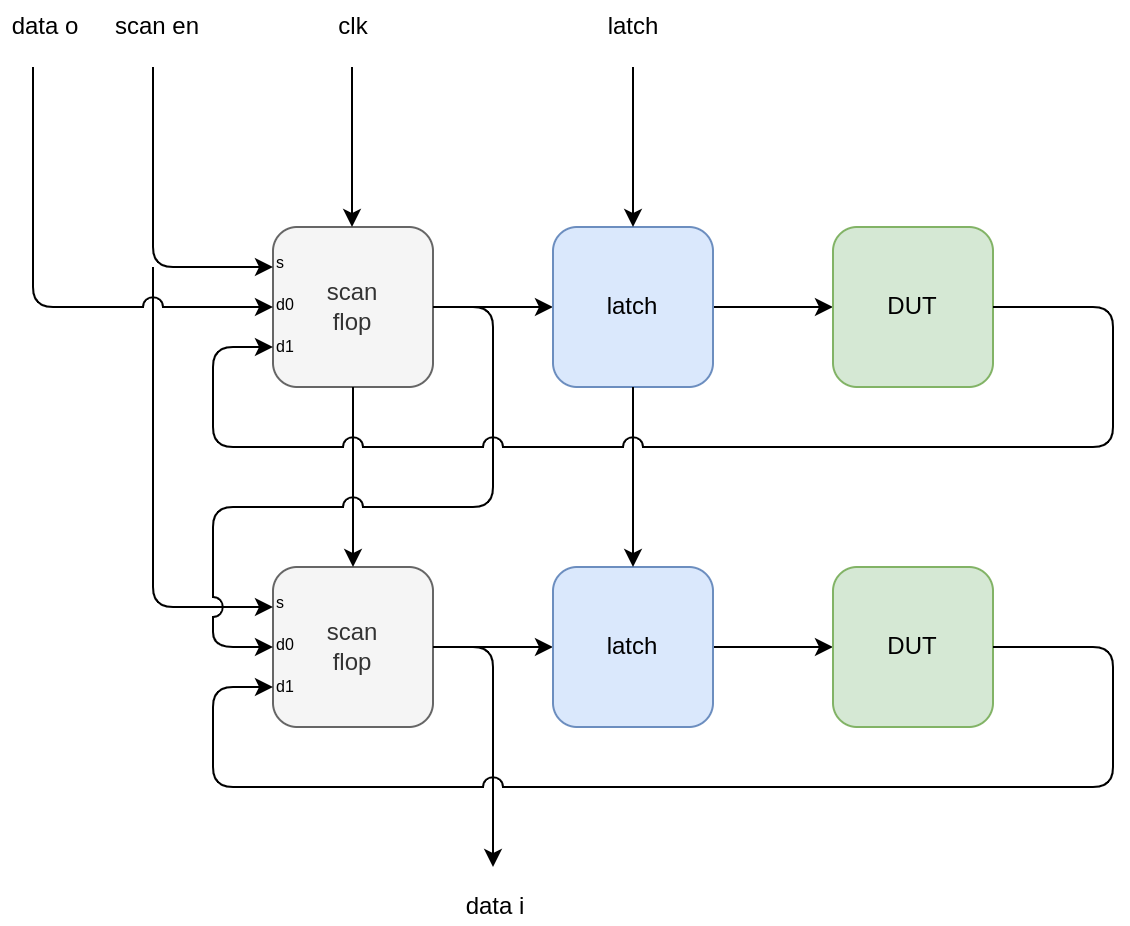
\includegraphics[width=\columnwidth]{./Figs/scanchain_block_diagram.png}
\caption{A simplified view of 2 designs in the chain.}
\label{fig:simplified_view_2_designs}
\end{figure}

Each design sends data into the scan flops secondary input and receives input from the output of the flop via a latch.
The chain is built~\cite{updateiodesign} by sending data from the output of the previous scan flop into the next scan flops’s primary input.

This arrangement allows the loading of data into any of the designs, and then capturing the output and clocking that through the rest of the chain to the output.

While relatively easy to implement, the downside is the latency.
The more designs in the chain, the longer it takes to send and receive data.
For example, assuming a \qty{50}{\MHz} scan chain clock, 250 designs with 8 inputs and 8 outputs, the maximum refresh rate is $\qty{50}{\MHz} / (8 \times 250) = \qty{25}{\kHz}$.

TT01’s scan chain was embedded into each design, which meant that a user could unintentionally remove it, breaking the chain.
This risk was mitigated with a formal~\cite{tinytapeoutscan} equivalence check---proving the chain was present in the submitted design.
For TT02 and TT03, the scan chain was separated into a separate macro block that the user can’t modify.

\begin{figure}[!t]
\centering
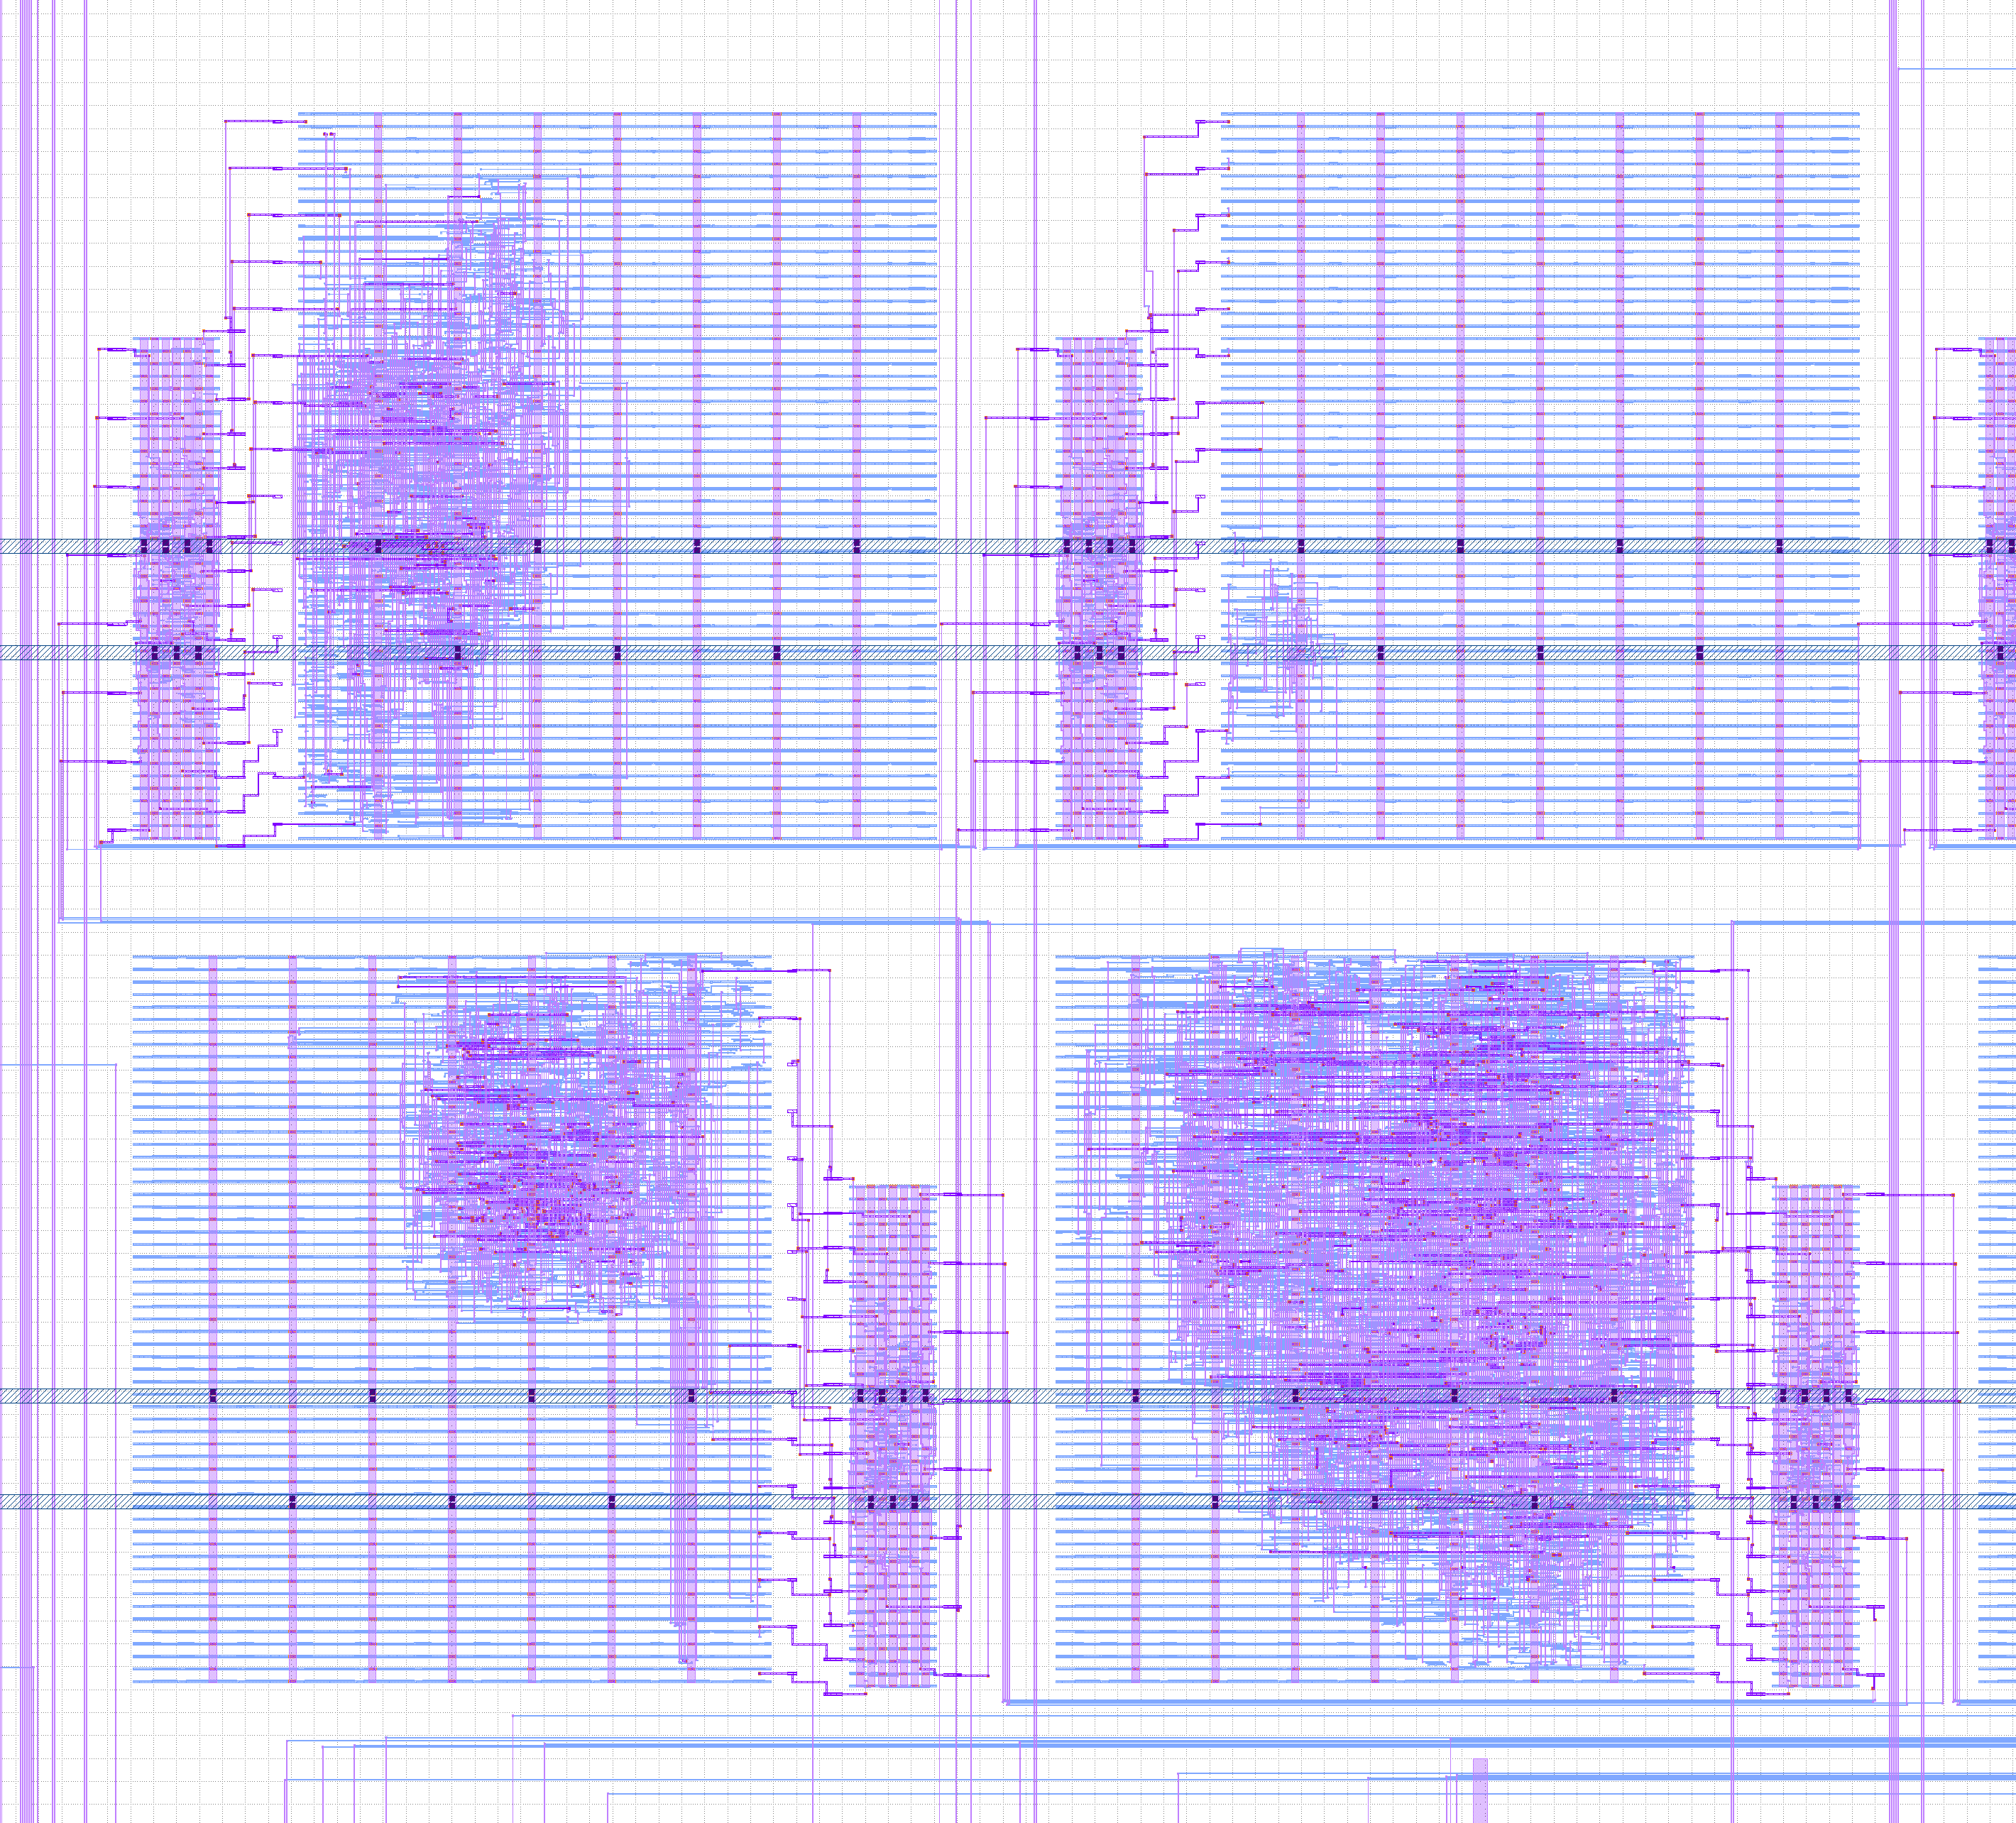
\includegraphics[width=\columnwidth]{./Figs/tt02_gds_zoom.png}
\caption{TT02 designs with separate scan chain blocks.}
\label{fig:TT02_separate_scan_blocks}
\end{figure}


Another concern was hold violations due to the large number of serially connected flops and potentially large clock skews due to long signal wires.  This was mitigated by reclocking the output data with a negedge flop, providing substantially more hold margin.

After static timing analysis (STA) it was discovered that the clock duty cycle could change substantially due to the \(500\) sequential clock drivers. Depending on the clock buffers and capacitance between each design, the clock duty cycle could either increase or decrease, with this effect accumulated over the chain.

For TT01 and TT02 each design used two clock buffers, with the internal flops driven after the first buffer.
TT03 used inverting clock buffers, with only one between the clock in and out. Fig. ~\ref{fig:TT02_vs_TT03} shows a comparison between the TT02 and TT03 clock buffer designs.  By inverting the clock between each design, any asymmetry in the clock pulse is evenly spread across the negative and positive cycles.

\begin{figure}[!t]
\centering
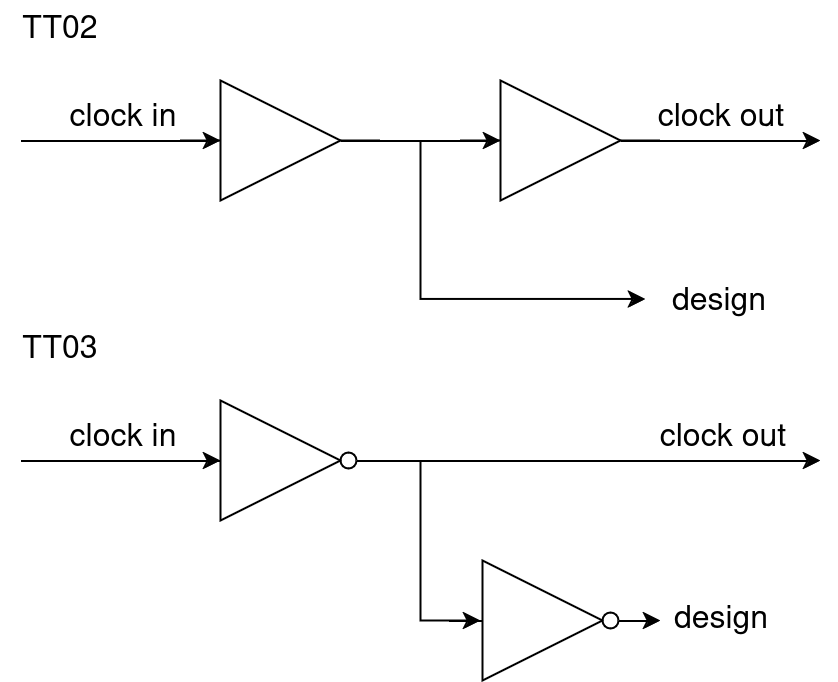
\includegraphics[width=\columnwidth]{./Figs/tt02 vs tt03 scanchain clock.png}
\caption{TT03 buffers the output from the clock network into each design. Clock polarity is alternated between designs to minimize asymmetry between positive and negative cycles.}
\label{fig:TT02_vs_TT03}
\end{figure}

The verification effort~\cite{verificationmd} was broad and included a community review, register transfer level (RTL) and gate level (GL) simulation, Formal Verification\cite{sby}, STA, layout vs schematic (LVS), DRC, and device level static verification~\cite{cvc}.
